%%
%%
%%      SECTION: SENSITIVITY
%%

%% \begin{figure}[htpb]
%% \begin{center}
%% %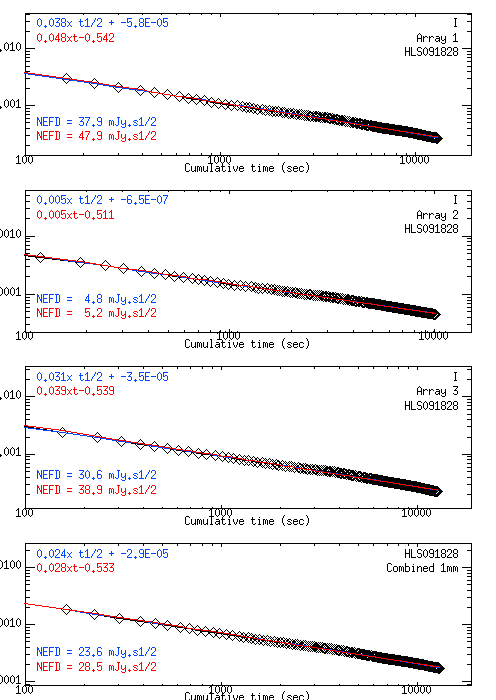
\includegraphics[clip, angle=0, scale =
%% %  0.5]{Figures/NEFD_HLS091828_20170226s415_FXDC0C1_GaussPhot.png}
%% %\includegraphics[clip, angle=0, scale = 0.5]{Figures/nefd_mpfit_HLS091828.eps}
%% \includegraphics[clip, angle=0, scale = 0.4]{Figures/HLS_fit.eps}
%% \includegraphics[clip, angle=0, scale = 0.4]{Figures/HLS_residuals.eps}
%% \caption{Sensitivity on \hls\ vs time of integration. Two power laws are fit:
%%   one with fixed slope $t^{1/2}$ that provides the estimate of the NEFD, one
%%   with a free slope $t^\beta$ to monitor the departure of noise integration from
%%   the canonical $t^{1/2}$. These data come from the integration on \hls\ during
%%   Run9. The difference between the 1 and 2~mm integration time comes from the
%%   density of KIDs in the FOV.}
%% \label{fig:nefd_vs_t}
%% \end{center}
%% \end{figure}

%% {\bf The specs/goals ``NEFD on X \% of pixels'' should be understood as : we have
%% XX\% valid pixels, and with these pixels, we have an NEFD of YY. We should not
%% discard some fraction of our pixels and estimate an NEFD on this subset.}\\

\hls is moderately faint source, expected to be below 100~mJy at 1mm and
XX~mJy at 2mm {\bf check values in NIKA1 paper + use SED for predictions in
  NIKA2's bands}. This source was chosen for its flux and its availability during
Run9 for long integration. It has been observed for XX hours in total over three
nights.


\subsection{Observations}

As part of the NIKA2 Science Verification that took place in February 2017, we
observed an area of 185~arcmin$^2$, centered on \hls, (a lensed dusty galaxy at
z=5.24 \cite{combes2012}) during about 9~hours. The scans were 8x5~arcmin$^2$,
alternatively oriented in (ra,dec), (dec,ra), (az,el), (el,az).\\

The MoU defines the NEFD:  \emph{The Noise Equivalent Flux Density (NEFD)
  is the $1\,\sigma$ sensitivity in one second of effective on-source telescope
  integration time after the absolute calibration has been performed (i.e. after
  beam efficiency and opacity corrections). It is appropriate for 2 mm of
  precipitable water vapor (pwv) content in the atmosphere and 60 degrees
  elevation source. It refers to the inverse variance of the noise on the flux
  measurement of a point-source, averaged over the valid receiver pixels}.

IRAM has its own time estimator that will compute the ``effective NEFD'',
provided we give the ``detector NEFD'' and a fraction of valid KIDs. We must be
careful not to mix both, which has been the case in several ways. We must not
mix the intuitive definition of the NEFD and that of the mapping speed as well :
in short, NIKA2's NEFD must be the same as NIKA's NEFD, but NIKA2's larger FOV
improves the mapping speed. All this was hidden in the definition of $\eta$ in
the previous version of this doc that I hope to clarify here.\\

To compute the instrumental NEFD (hereafter NEFD), we must compute the
integration time on the source. This time is the total time spent by detectors
measuring the source, \emph{not} by the matrix footprint. Let's be more
specific: if the source is in the focal plane, but on a place where no KID is
valid, the integration time is zero. There are 3 ways to estimate the time of
integration. We introduce them in the following 3 subsections and compare them
on Fig.~\ref{fig:time_comparison}.

\subsubsection{Time of integration from the density of samples}

Let's take a map of resolution $r$. The number of hits in the central pixel on
the source $N_h(r)$ leads to:

\begin{equation}
t_{int} = \frac{N_h(r)}{\nu}\frac{1}{N_{kids\,per\,pixel}}
\end{equation}

Suppose we stay fixed on the source (no movement at all) during a time $t_{obs}$, and $r$ is such that
there is only one KID staring at the source, then

\begin{equation}
t_{int} = \frac{1}{\nu}t_{obs}\times\nu = t_{obs}
\end{equation}

Suppose there are two kids per pixels, then the number of hits is twice as large
while $t_{obs}$ remains the same. In practice, this factor
$N_{kids\,per\,pixel}$ is difficult to estimate exactly because it depends on the
scanning strategy and the repartition of KIDs accross the FOV. In practice, we
are bound to compute averages and thus to estimate the average number of KIDs
per map pixel which is 

\begin{equation}
N^{avg}_{kids\,per\,pixel} = r^2/g^2
\end{equation}

where $g$ is the grid step of a matrix. Indeed, the total surface coverged by
$N_{kids}$ detectors is $S = N_{kids}g^2$ and there are $S/r^2$ map pixels in
this surface. So, the integration time on the source is finally

\begin{equation}
t_{int} = \frac{N_h(r)}{\nu}\frac{g^2}{r^2}\,.
\label{eq:t_int}
\end{equation}

Another justification of this formula is that $N_h(r)/r^2$ is the density of
samples in hits/arcsec$^2$ and $g^2$ is the inverse of the number of KIDs per
arcsec$^2$. For the combined 1mm, we must divide by 2 because both matrices
observe the same area at the same time:

\begin{equation}
t^{1mm}_{int} = \frac{1}{2}\frac{N_h(r)}{\nu}\frac{g^2}{r^2}\,.
\label{eq:t_int_1mm}
\end{equation}

So finally:

\begin{equation}
NEFD = \sigma \sqrt{t_{int}}
\label{eq:nefd_t_int}
\end{equation}

With this definition in hand, assuming we have only $N_{valid}$ kids in a focal
plane of $N_{full}$ KIDs in theory, we can, as a rule of thumb, estimate
the required time of integration required to reach a sensitivity
$\sigma_{target}$. Let's call $\eta = N_{valid}/N_{full}$ the fraction of valid
KIDs of the matrix. To reach the same number of hits per map pixels, with the
same scanning strategy, the total integration time must be $1/\eta$ time larger,
hence : 

\begin{equation}
t_{astronomer} = \left(\frac{NEFD}{\sigma_{target}}\right)^2\frac{1}{\eta}
\label{eq:t_astro}
\end{equation}

\subsubsection{Time of integration from the matrix footprint}

One can also think of the ``time spent on the source'', for a full matrix
(ie. all valid KIDs), as the time when the source is inside the circular
footprint of the matrix. During a scan, it's easy to count how much time the
source is at a distance from the FOV center that is larger than the FOV
radius. Let's call this time $t_{geom}$. However, because the map is produced
with only a fraction $\eta$ of valid KIDs, the effective integration time on the
source is $\eta$ times smaller than $t_{geom}$. Hence:

\begin{equation}
NEFD = \sigma \sqrt{t_{geom}\eta}
\label{eq:nefd_t_geom}
\end{equation}


\subsubsection{Time of integration from the flux estimator}

The NEFD is defined as the noise ``per beam'', the uncertainty on the estimation
of the flux of a point source. The estimation of a point source flux is given by
the fit of a gaussian profile, that in the case of white noise reduces to:

\begin{equation}
\hat{\phi} = \frac{1}{\sum_p g_p^2}\sum_p g_p m_p\,,
\label{eq:phi_def}
\end{equation}

and whose variance is

\begin{equation}
\sigma_\phi^2 = \left(\frac{1}{\sum_p g_p^2}\right)^2\sum_p g_p^2\sigma_p^2\,.
\label{eq:sigma_phi_def}
\end{equation}

In the case of white noise and considering the equivalent of the
uniform full matrix of the NEFD definition: $\sigma_p = \sigma/\sqrt{N_p}$,
where $\sigma$ is the standard deviation of 1 sample and $N_p$ is the number of
hits in pixel $p$. Accounting for the sampling frequency, it reads

\begin{eqnarray}
\sigma_\phi^2 &=& \frac{\sigma}{\nu}\left(\frac{1}{\sum_p g_p^2}\right)^2\sum_p \frac{g_p^2}{t_p}\,, \nonumber\\
&=&\frac{\sigma}{\nu}\frac{1}{t_{beam}}\,
\label{eq:sigma_phi_def_2}
\end{eqnarray}

where $t_{beam}$ is homogeneous to a time and is such that $\sigma_\phi$ goes
like $1/\sqrt{t_{beam}}$.\\


\begin{figure}
\begin{center}
\includegraphics[clip, angle=0, scale =0.8]{Figures/Pluto_time_of_integration.eps}
\caption{Comparison between three estimators of the time of integration on the
  source during Pluto's observation (Run9). To a few percent, the 3 estimators
  give compatible estimations.}
\label{fig:time_comparison}
\end{center}
\end{figure}


%% Note: there is no way to be perfectly precise on the estimation of these
%% parameters, in all circumstances, on the edges of any matrix, for potential
%% areas covered by A1 and not A3 (or just less). Like in any case, we must live
%% with this, focus on the main area of each scan and forget about edge effects.

\subsection{History and confusions}

In the past few days, we have re-examined these definitions, and several
mistakes were made:

\begin{itemize}
\item at some point, the {\tt nk\_map\_photometry.pro} that is supposed to give
  the correct ``time'', rather than giving $t_{int}$ as defined in
  Eq.~(\ref{eq:t_int}) was giving $\eta t_{int}$.
\item When questioning this relation, we confused $t_{int}$ and $t_{obs} = t_{int}/\eta$. While
  the dependence on the grid step and the map resolution was accounted for in
  average, it was not the correct time to consider to compute the NEFD as defined in
  the MoU (a.k.a detector NEFD, letting $\eta$ as another parameter in IRAM's
  time estimator).
\item In the end, the final NEFD we must give to IRAM are those that we
  published but increased by a factor $1/\sqrt{\eta}$.
\end{itemize}



\subsection{Data processing}

The data were decorrelated using the {\tt common-monde-one-block} method
(cf.~\ref{se:cm1blck}), masking a disk of 60~arcsec radius centered \hls.  The
scans have been combined with standard inverse noise weighting. The noise in
each map pixel is derived from the rms of the background corrected by the square
root of the number of observations per pixel (N1). If the noise was perfectly
gaussian, the distribution of the map signal over this noise estimate (far from
the source) would be a normalized gaussian. In practice, this leads to gaussians
that 1.6 and 1.5 larger. We therefore increase our noise estimate (N1) by these
factors to derive our final estimates. Should the extra sources that pop up in
the field contribute to this estimate, they would only make our estimate more
conservative.

\subsection{NEFD Methods 1 and 2: deep integration}

%% \input{hls_1mm.tex}
%% \input{hls_2mm.tex}
%% \input{Pluto.tex}

These data can be used to derive the NEFD in several ways. One is to fit the
evolution of the uncertainty on the flux of the source $\sigma_\phi$ with the
integration time. Another one is to produce jackknife maps with the data and to
measure the uncertainty on the flux in the end, while estimating the time of
integration. Depending on what definition of the time of integration we take, we
might get slightly varying answers, we'll come back to this later one. However,
we must note right now that the assumption that the sensitivity should go like
$1/\sqrt{t}$ needs clarification. This can only be true if scans are co-added
with equal noise weights and are observed under the same conditions of opacity
and elevation. Otherwise, corrections must be taken into account. Indeed, 

\begin{equation}
\sigma = NEFD_0e^{\tau/\sin\delta}\sqrt{t}
\label{eq:sigma_nefd}
\end{equation}

and scans are coadded with inverse variance weighting, so the combined flux is:

\begin{equation}
\phi = \frac{1}{\sum_n 1/\sigma_n^2}\sum_n\frac{\phi_n}{\sigma_n^2}
\end{equation}

whose variance is

\begin{equation}
\sigma^2 = \frac{1}{\sum_n 1/\sigma_n^2}
\end{equation}

which, according to Eq.~(\ref{eq:sigma_nefd}) becomes

\begin{equation}
\sigma^2 = \frac{NEFD_0^2}{\sum_{n}t_n e^{-2\tau_n/\sin\delta_n}}\,.
\label{eq:sigma_tau_w8}
\end{equation}

If the opacity and the elevations are the same for all scans, we recover the
integration like $\sqrt{t}$. In general, if the observing conditions vary, we
must fit the integrated sensitivity vs the effective time $\sum_{n}t_n
e^{-2\tau_n/\sin\delta_n}$ in order to recover an unbiased estimate of
$NEFD_0$. Luckily enough, we have observations of Pluto in very stable
atmospheric conditions and at quasi constant elevation. This will allow us to
check this formalism against more intuitive and direct definitions. We can also
extract from the scans on \hls those that were under stable opacity conditions
and at high and quasi-constant elevation as a confirmation of our final
estimates. The other regimes will help us derive uncertainties our estimates.\\

\begin{figure}[htpb]
\begin{center}
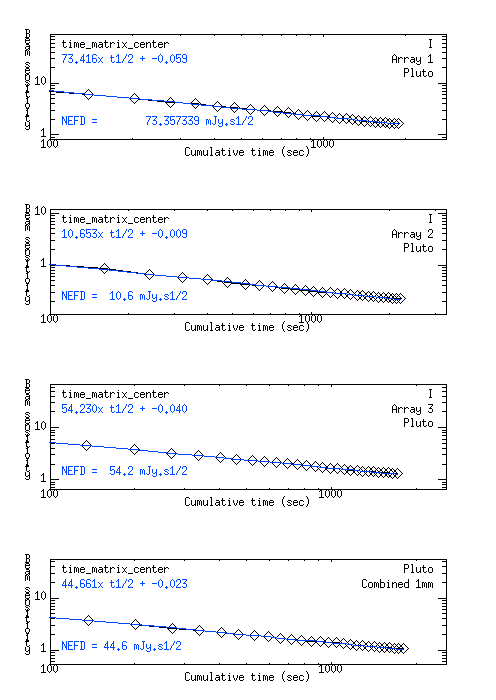
\includegraphics[clip, angle=0, scale=0.4]{Figures/Pluto_8_sigma_vs_time_matrix_center.png}
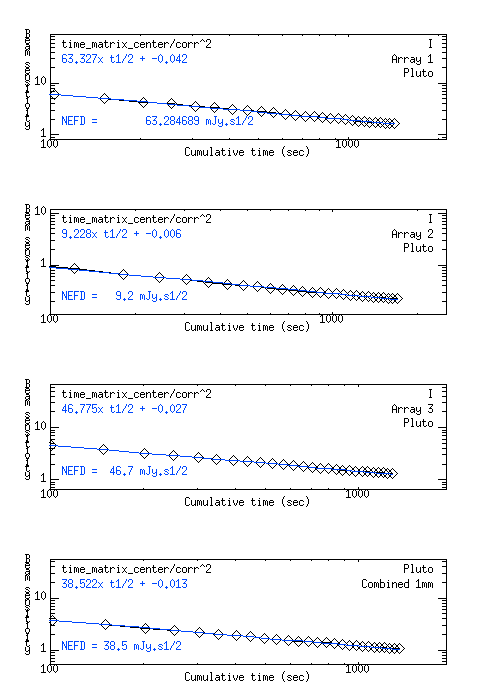
\includegraphics[clip, angle=0, scale=0.4]{Figures/Pluto_8_sigma_vs_time_matrix_center_tau_w8.png}
\caption{\emph{Left:}$1\,\sigma$ sensitivity vs $t_{int}$ during observations of Pluto, {\bf
  without correction for elevation or opacity}. \emph{Right:} Same fit but this
  time considering the effective time, weighted by opacity and elevation as in Eq.~(\ref{eq:sigma_tau_w8}).}
\label{fig:Pluto_8_sigma_vs_time_matrix_center}
\end{center}
\end{figure}


\begin{figure}[htpb]
\begin{center}
\includegraphics[clip, angle=0, scale=0.4]{Figures/Pluto_5_opacity.eps}
\includegraphics[clip, angle=0, scale=0.4]{Figures/Pluto_5_elevation.eps}
\includegraphics[clip, angle=0, scale=0.4]{Figures/HLS091828_5_opacity.eps}
\includegraphics[clip, angle=0, scale=0.4]{Figures/HLS091828_5_elevation.eps}
\caption{Opacities and elevations during observations of Pluto and \hls. While
  conditions were stable both in opacity and elevation for Pluto, it was not the
case for \hls.}
\label{fig:pluto_opacities}
\end{center}
\end{figure}

\paragraph{Pluto.} We have 28 scans of Pluto, for a total
integration time of XX at 1mm and XX at
2mm. Fig.~\ref{fig:Pluto_8_sigma_vs_time_matrix_center} shows how the
$1\,\sigma$ sensitivity decreases with $t_{int}$. Considering the small
variations of opacity and elevation during these observations of Pluto
(Fig.~\ref{fig:pluto_opacities}), we can derive an average correction
$exp(-\tau/\sin\delta) = exp(-0.07/\sin(30^\circ)) = 0.87$. This leads to zenith
$NEFD_0^{1mm} = 38.8$ and $NEFD_0^{2mm} = 9.2$\,mJy.s$^{-1/2}$. Using the
jackknife maps and applying the same opacity-elevation correction, one gets
$NEFD_0^{1mm}=38.0$ and $NEFD_0^{2mm}=8.96$.

In light what is discussed in the previous paragraph, if we fit the sensitivity
vs $\sum_{n}t_n e^{-2\tau_n/\sin\delta_n}$, we obtain $NEFD_0^{1mm} = 38.5$ and
$NEFD_0^{2mm}=9.2$. These value are summarized in
tables~\ref{tab:nefd_stable_1mm} and \ref{tab:nefd_stable_2mm}. All these
numbers are obtained with the standard reduction method, a.~k.~a. {\tt
  common\_mode\_one\_block, (CMB)}. If we further subtract a polynomial of order
5 per subscan after this decorrelation (still masking the source), we improve
the results as reported in the tables, while not changing the measured fluxes of
Pluto and HLS (tab.~\ref{tab:fluxes}). We therefore do not change the
calibration with this extra filtering, so the gain in sensitivity does come from
better noise subtraction.

\paragraph{\hls.} While we have an overall
longer integration on \hls, it was acquired during distinct periods, over
varying elevation and different (albeit almost constant by plateau)
opacities (Fig.~\ref{fig:hls_opacities}). Still, performing the same analyses, we obtains the results presented
in tables~\ref{tab:nefd_stable_1mm} and \ref{tab:nefd_stable_2mm}. The values
obtained from the fit vs $1/\sqrt{t}$ are recalled to illustrate the impact of
the opacity-elevation correction on this estimator on \hls\ data. One should
focus on the values derived from the Jackknivfe maps and thoses including the
opacity-elevation correction $1/\sqrt{t_{eff}}$: these values are in very good
agreement when derived from the same reduction method, and in good agreement
between Pluto and \hls.\\

{\bf Conclusion}: while uncertainties on these values should be further
investigated, the good agreement between alternative estimates and at the same
time their differences indicate that they should be valid at about $\pm 1$\,mJy.s$^{1/2}$.
{\bf With these two estimators (fit vs time of integration and
  Jackknife), we find zenith $NEFDs$ below 35 and 9\,mJy.s$^{1/2}$ at 1 and
  2\,mm respectively.} While less intuitive, the more rigourous definition of
the integration time that enters the estimation of the flux, $t_{beam}$, leads to
  slightly different values. It improves by 5\% at 1\,mm, i.e. puts the upper limit at 33.4, but
  degrades the 2\,mm value by the same amount and raise the upper limit to 9.3.

\begin{table}
\begin{tabular}{|l|l|l|l|l|}
\hline
$NEFD_0^{1mm}$~mJy.s$^{1/2}$ & \multicolumn{2}{|c|}{Pluto} & \multicolumn{2}{|c|}{\hls}\\
\hline
Red.~method             & CMB     & CMB+poly5     & CMB & CMB+poly5\\
\hline
$\sim 1/\sqrt{t}$       & 38.8  & 34.3  & 41.7 & 38.2\\
$JK$                    & 35.9  & {\bf 34.7}  & 33.8 & {\bf 33.6} \\
$\sim 1/\sqrt{t_{eff}}$ & 38.5  & {\bf 32.8}  & 37.5 & {\bf 34.4} \\
\hline
\hline
\end{tabular}
\caption{Zenith NEFD's in stable elevation and atmospheric conditions on Pluto
  and \hls\ at 1mm.}
\label{tab:nefd_stable_1mm}
\end{table}

\begin{table}
\begin{tabular}{|l|l|l|l|l|}
\hline
$NEFD_0^{2mm}$~mJy.s$^{1/2}$ & \multicolumn{2}{|c|}{Pluto} & \multicolumn{2}{|c|}{\hls}\\
\hline
Red.~method             & CMB     & CMB+poly5     & CMB & CMB+poly5\\
\hline
$\sim 1/\sqrt{t}$       & 9.3 & 8.0 & 9.8  & 8.5\\
$JK$                    & 8.8 & {\bf 7.7} & 8.3  & {\bf 7.6} \\
$\sim 1/\sqrt{t_{eff}}$ & 9.2 & {\bf 8.2} & 9.4  & {\bf 8.2} \\
\hline
\hline
\end{tabular}
\caption{Zenith NEFD's in stable elevation and atmospheric conditions on Pluto
  and \hls\ at 2mm.}
\label{tab:nefd_stable_2mm}
\end{table}

\begin{table}
\begin{tabular}{|l|l|l|l|l|}
\hline
Fluxes (mJy) & \multicolumn{2}{|c|}{Pluto} & \multicolumn{2}{|c|}{\hls}\\
\hline
Red.~method  & CMB           & CMB+poly5     & CMB           & CMB+poly5\\
\hline
1\,mm        & $15.0\pm 1.1$ & $13.6\pm 0.9$ & $85.2\pm 0.4$ & $85.4\pm 0.4$\\
2\,mm        & $5.0\pm 0.2$  & $5.0\pm 0.2$  & $14.9\pm 0.1$ & $14.9\pm 0.1$\\
\hline
\hline
\end{tabular}
\caption{Measured fluxes of Pluto and \hls\ with two data reduction methods. The
  extra subtraction of polynomial of order 5 per subscan while masking the
  source does not subtract power to the source, hence the derived sensitivities
  with this methods do not need to be recalibrated.}
\label{tab:fluxes}
\end{table}

%% Tab.~\ref{tab:nefd}. Fig.~\ref{fig:nefd_vs_t} shows the decrease of the
%% uncertainty on the measured flux at the center of the map as a function of
%% time. We either fit a power law or fix the power law to -0.5 and fit only the
%% amplitude. Uncertainties on these values have been estimated via a bootstrap
%% method: we randomize the scans and derive the standard deviation of the average
%% of $n$ scans for any $n$ between 1 and the total number of scans. This gives us
%% an estimate of the uncertainty on $\sigma_\phi$ for a time of integration
%% corresponding to $n$ scans. Strictly speaking, all the scans do not have the
%% exact same duration, but the difference is negligible here.

%% \begin{table}
%% \begin{tabular}{|l|l|l|l|l|}
%% \hline
%% Array & Free power law & Fixed power law $t^{-0.5}$ & Jackknife & Instrument \\
%% \hline
%% A1       & $47.9$ mJy.s$^{-0.54}$ & $37.9$ mJy.s$^{1/2}$ & 35.6 mJy.s$^{1/2}$ & $33.3$ (5) mJy.s$^{1/2}$\\
%% A2       & $5.2$  mJy.s$^{-0.51}$ & $4.8$  mJy.s$^{1/2}$ & 5.7  mJy.s$^{1/2}$ & $5.8$  (5) mJy.s$^{1/2}$\\
%% A3       & $38.9$ mJy.s$^{-0.54}$ & $30.6$ mJy.s$^{1/2}$ & 30.4 mJy.s$^{1/2}$ & $28.4$ (4) mJy.s$^{1/2}$\\
%% A1 \& A3 & $28.5$ mJy.s$^{-0.53}$ & $23.6$ mJy.s$^{1/2}$ & 22.4 mJy.s$^{1/2}$ & $21.1$ (3) mJy.s$^{1/2}$\\
%% \hline
%% \end{tabular}
%% \label{tab:nefd}
%% \caption{Noise integration with observation time and associated derivations of
%%   the NEFD. These values do not account for the extra {\color{red} \bf XXXX \%}
%%   uncertainty on absolute calibration.}
%% \end{table}
%       33.325263       5.2024647
%       28.397230       4.5723151
%       21.143376       4.1538804
%       5.7628233       3.3094792

%% 
%% \begin{figure}
%% \begin{center}
%% 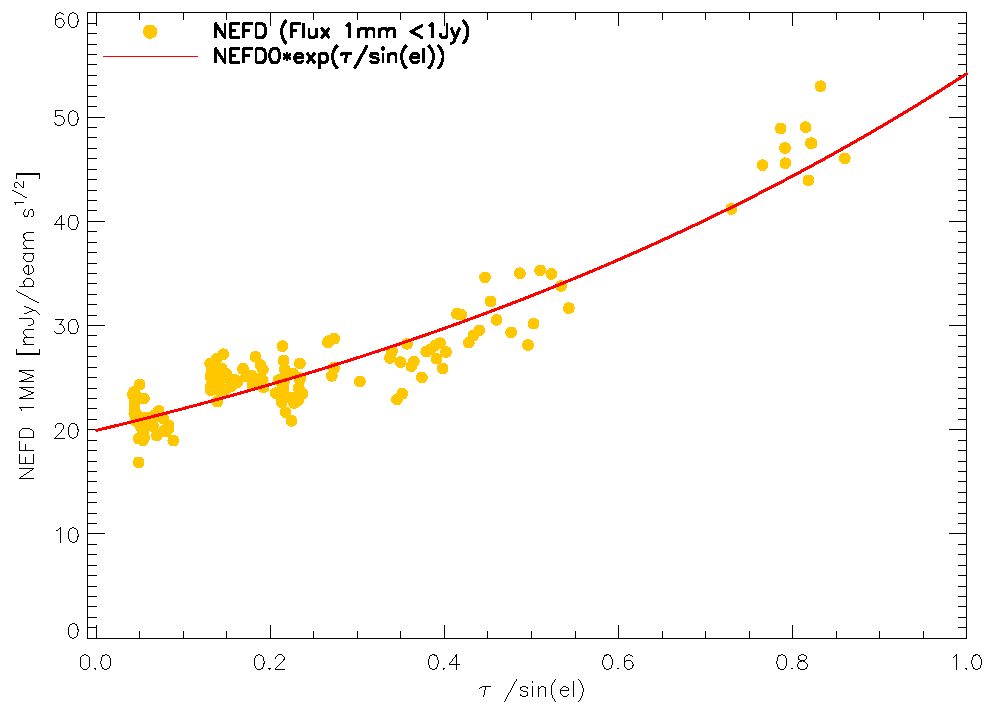
\includegraphics[clip, angle=0, scale =0.8]{Figures/NEFDIndScans/nefd_1mm_R9_F1_tau_run22_23.pdf}
%% 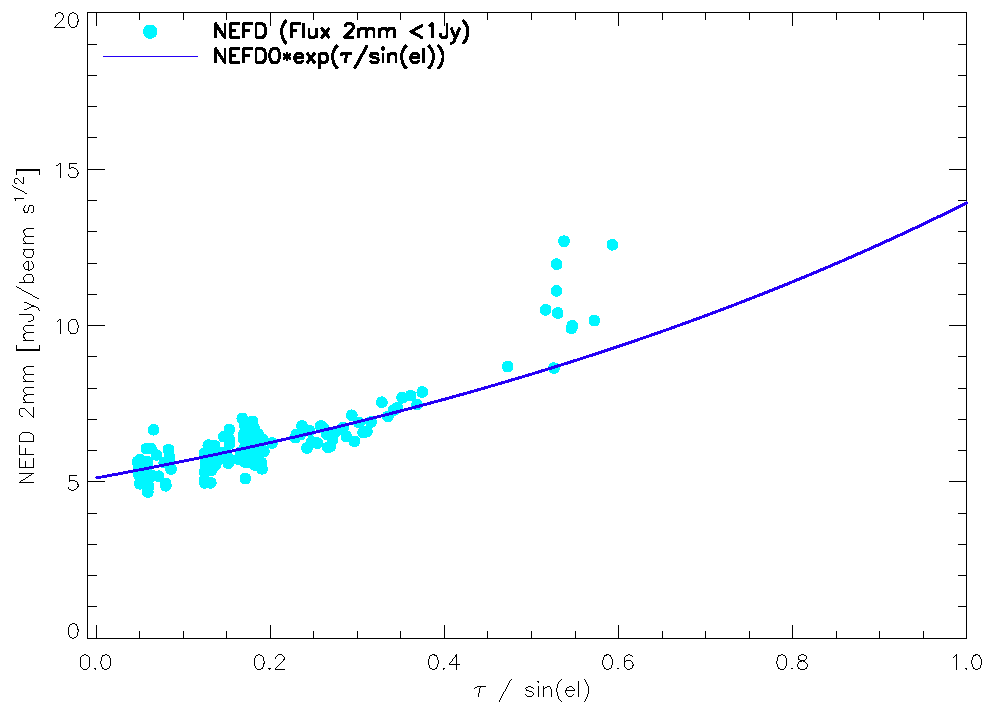
\includegraphics[clip, angle=0, scale =0.8]{Figures/NEFDIndScans/nefd_2mm_R9_F1_tau_run22_23.pdf}
%% \caption{Measured NEFD as a function of atmospheric background for the 1 (top) and 2 (bottom) mm channels. We also show in the plots the expected NEFD evolution with atmospheric background as solid curves.}
%% \label{fig:nefdvsbackground}
%% \end{center}
%% \end{figure}
%% 
%% \subsection{NEFD Method 3: scan NEFD vs opacity and air mass}
%% \begin{figure}
%% \begin{center}
%% 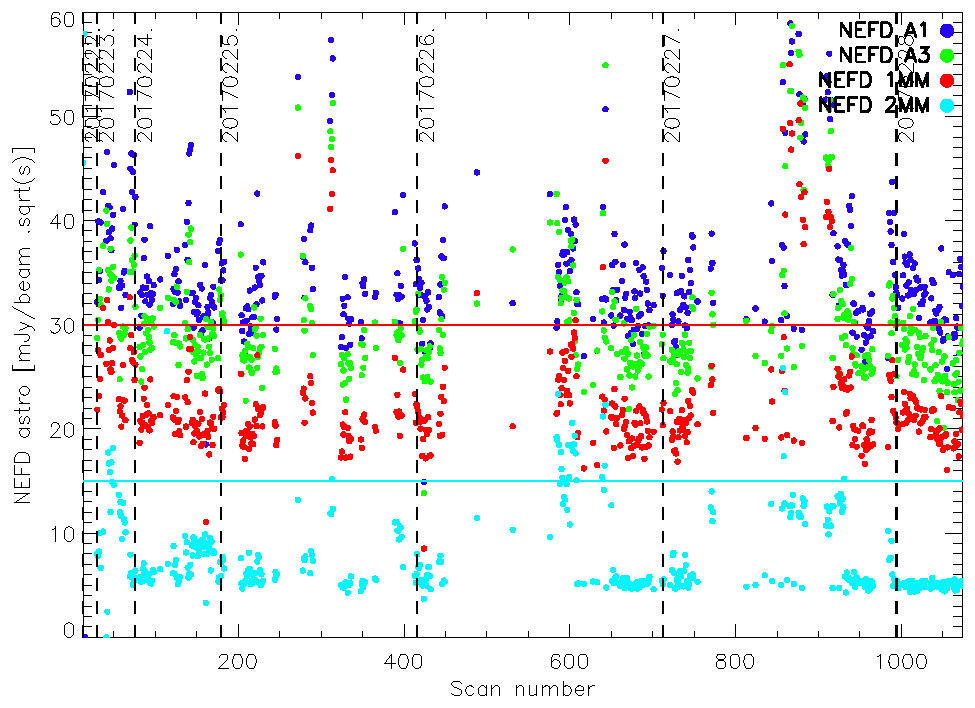
\includegraphics[clip, angle=0, scale =0.8]{Figures/NEFDIndScans/nefd_evol_run22.pdf}
%% \caption{Evolution of the measured instrument NEFD across scans for N2R9.}
%% \label{fig:nefdvsscans}
%% \end{center}
%% \end{figure}
%% 
%% \begin{figure}
%% \begin{center}
%% 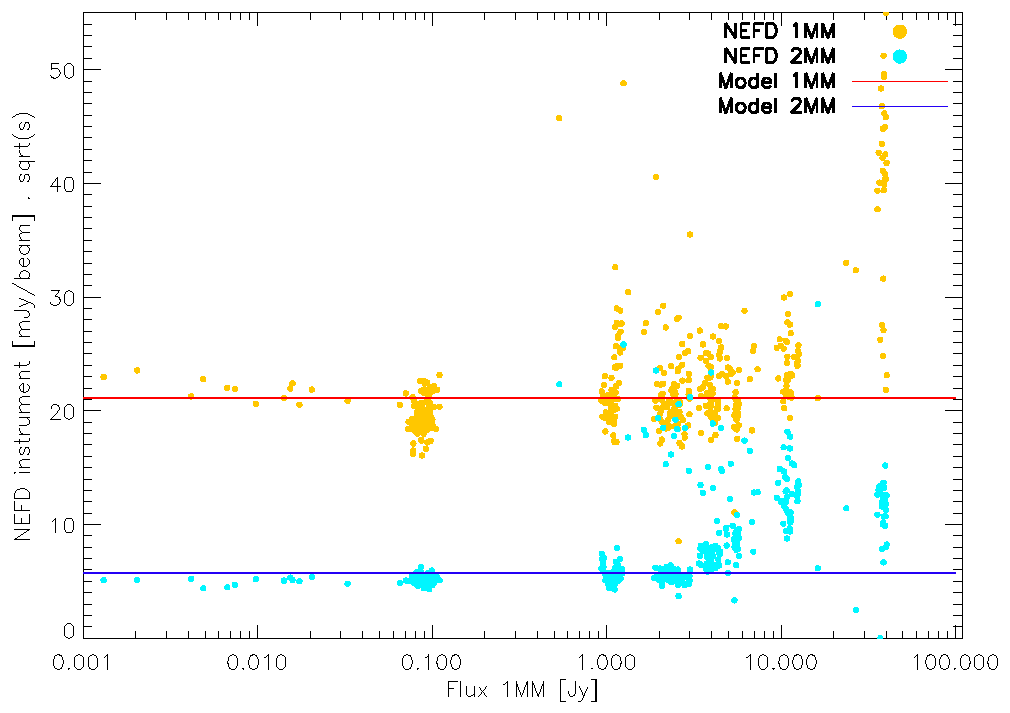
\includegraphics[clip, angle=0, scale =0.8]{Figures/NEFDIndScans/nefd_flux1mm_run22.pdf}
%% \caption{Measured instrument NEFD as a function of the flux of the source.}
%% \label{fig:nefdvsflux}
%% \end{center}
%% \end{figure}
%% \begin{figure}
%% \begin{center}
%% 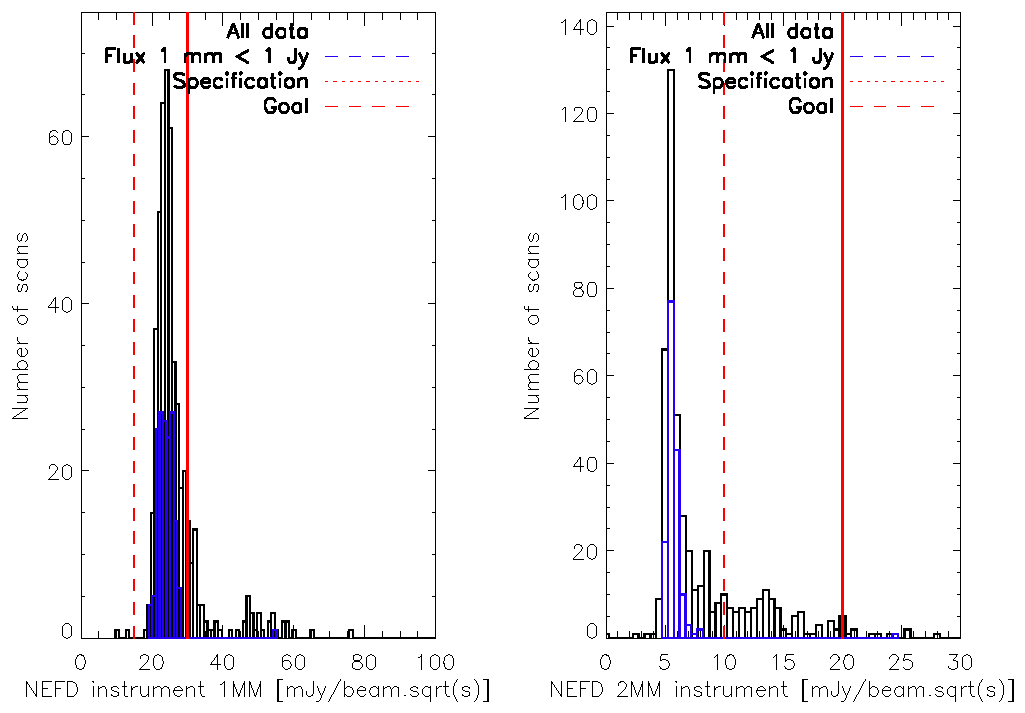
\includegraphics[clip, angle=0, scale =0.8]{Figures/NEFDIndScans/hist_nefd_ref_run22.pdf}
%% \caption{Histogram of the measured reference NEFD across the N2R9 for the 1 (right) and 2 (left) mm channels.}
%% \label{fig:nefdhist}
%% \end{center}
%% \end{figure}
%%  
%% 
%% In this section we investigate the astronomer NEFD as a function of the
%% atmospheric opacity and air mass. Figure~\ref{fig:nefdvsbackground} shows the
%% measured NEFD, which we refer to as astronomer NEFD, for the 1 and 2 mm as a
%% function of the measured atmospheric background in terms of $\tau/sin(El)$. The
%% atmospheric opacity was computed as discussed in Section~\ref{se:opacities}. We
%% observe that the increase of the astronomer NEFD is in agreement with what we
%% would expect for background dominated sensitivity. We observe however some
%% significant deviations from the curve. To investigate this issue we also show in
%% Figure~\ref{fig:nefdvsscans} the evolution of the background corrected NEFD,
%% hereafter instrument NEFD, across the N2R9 campaign for arrays A1 (blue), A3
%% (green) and A2 (cyan), and for the combination of A1 and A3 (red). We globally
%% obseve stable NEFD across the run, with A1 sensitivity being worse than for
%% A3. We also show the measured instrument NEFD as a function of the flux of the
%% source in the 1 mm channel in Figure~\ref{fig:nefdvsflux}. We observe that the
%% observed deviations in the instrument NEFD correspond mainly to the large flux
%% source scans. This is more obvious in Figure~\ref{fig:nefdhist} where we present
%% the histogram of the measured NEFD for 2 mm of pwv and at a elevation of 60
%% degrees, hereafter, reference NEFD, for the 1 and 2 mm channels.


